\documentclass{beamer}

% Theme
\usetheme{CambridgeUS}
\usepackage[utf8]{inputenc}
\usepackage{graphicx}

\definecolor{darkgreen}{rgb}{0.0, 0.5, 0.0}

% Title info
\title[Custom BIOS with coreboot]{How to Build Your Own BIOS Using coreboot}
\author{Reza Adinepour}
\date{\today}

\begin{document}
	
	% Title page with logo below the date
	\begin{frame}
		\titlepage
		\vspace{0.5cm}
		\centering
		
\includegraphics[width=2.5cm]{images/logo/logo.png} % Place logo.png in the same folder
	\end{frame}
	
	% Remove logo for all next slides
	\logo{}
	
	% Outline
	\begin{frame}{Outline}
		\tableofcontents
	\end{frame}
	
	% Section: Dependency Installation
	\section{Dependency Installation}
	\subsection{Git}
	\begin{frame}{Git}
		To build and configure coreboot, we need to install several packages:
		
		\begin{itemize}
			\item Development tools and version control
			\item Coreboot build dependencies
			\item Optional firmware tools
		\end{itemize}
		
		\vspace{0.4cm}
		\textbf{Step 1: Install Git (Ubuntu/Debian)}
		
		\begin{exampleblock}{Install git}
			\textcolor{blue}{\$} \texttt{sudo apt install git}
		\end{exampleblock}
		
		\textbf{Step 2: Verify Git installation}
		
		\begin{exampleblock}{Check version}
			\textcolor{blue}{\$} \texttt{git --version}
		\end{exampleblock}
	\end{frame}
	
	
	
	\begin{frame}{Git (Cont.)}
		\textbf{Step 3: Set user identity}

		\begin{exampleblock}{Set username}
			\textcolor{blue}{\$} \texttt{git config --global user.name "Reza Adinepour"}
		\end{exampleblock}
		
		\begin{exampleblock}{Set email}
			\textcolor{blue}{\$} \texttt{git config --global user.email "reza@example.com"}
		\end{exampleblock}
		
		\textbf{Step 4: Set default text editor (optional)}
		
		\begin{exampleblock}{Set vim as editor}
			\textcolor{blue}{\$} \texttt{git config --global core.editor "vim"}
		\end{exampleblock}
	\end{frame}
	
	
	
	
	
	
	
	\subsection{Python}
	\begin{frame}{Python}
		Python is usually pre-installed on most Linux distributions.
		
		\vspace{0.3cm}
		\textbf{Step 1: Check if Python is already installed}
		
		\begin{exampleblock}{Check Python version}
			\textcolor{blue}{\$} \texttt{python3 --version}
		\end{exampleblock}
		
		\textbf{If not installed, install Python manually:}
		
		\begin{exampleblock}{Install Python}
			\textcolor{blue}{\$} \texttt{sudo apt install python3 python3-pip}
		\end{exampleblock}
	\end{frame}
	
	
	
	
	
	\section{Coreboot Installation}
	\begin{frame}{Installing Coreboot}
		\textbf{Step 1: Install tools and libraries needed for coreboot}
		
		\begin{exampleblock}{Install build dependencies}
			\textcolor{blue}{\$} \texttt{sudo apt-get install -y bison \\
				\hspace*{3.4em}build-essential \\
				\hspace*{3.4em}curl \\
				\hspace*{3.4em}flex \\
				\hspace*{3.4em}gnat \\
				\hspace*{3.4em}libncurses-dev \\
				\hspace*{3.4em}libssl-dev \\
				\hspace*{3.4em}zlib1g-dev \\
				\hspace*{3.4em}pkgconf}
		\end{exampleblock}
	\end{frame}
	
	
	
	\begin{frame}{Installing Coreboot (Cont.)}
		\textbf{Step 2: Clone the official coreboot repository}
		
		\begin{exampleblock}{Clone coreboot}
			\textcolor{blue}{\$} \texttt{git clone https://review.coreboot.org/coreboot}
		\end{exampleblock}
		
		\textbf{Step 3: Enter the coreboot directory}
		
		\begin{exampleblock}{Enter directory}
			\textcolor{blue}{\$} \texttt{cd coreboot}
		\end{exampleblock}
		
		\textbf{Step 4: Initialize submodules}
		
		\begin{exampleblock}{Fetch submodules}
			\textcolor{blue}{\$} \texttt{git submodule update --init --recursive}
		\end{exampleblock}
	\end{frame}
	
	
	
	
	
	
	\begin{frame}{Installing Coreboot (Cont.)}
		\textbf{Step 5: Build the coreboot toolchain}
		
		\begin{exampleblock}{Build}
			\textcolor{blue}{\$} \texttt{make crossgcc-i386 CPUS=\$(nproc)}
		\end{exampleblock}
		
		\centering
		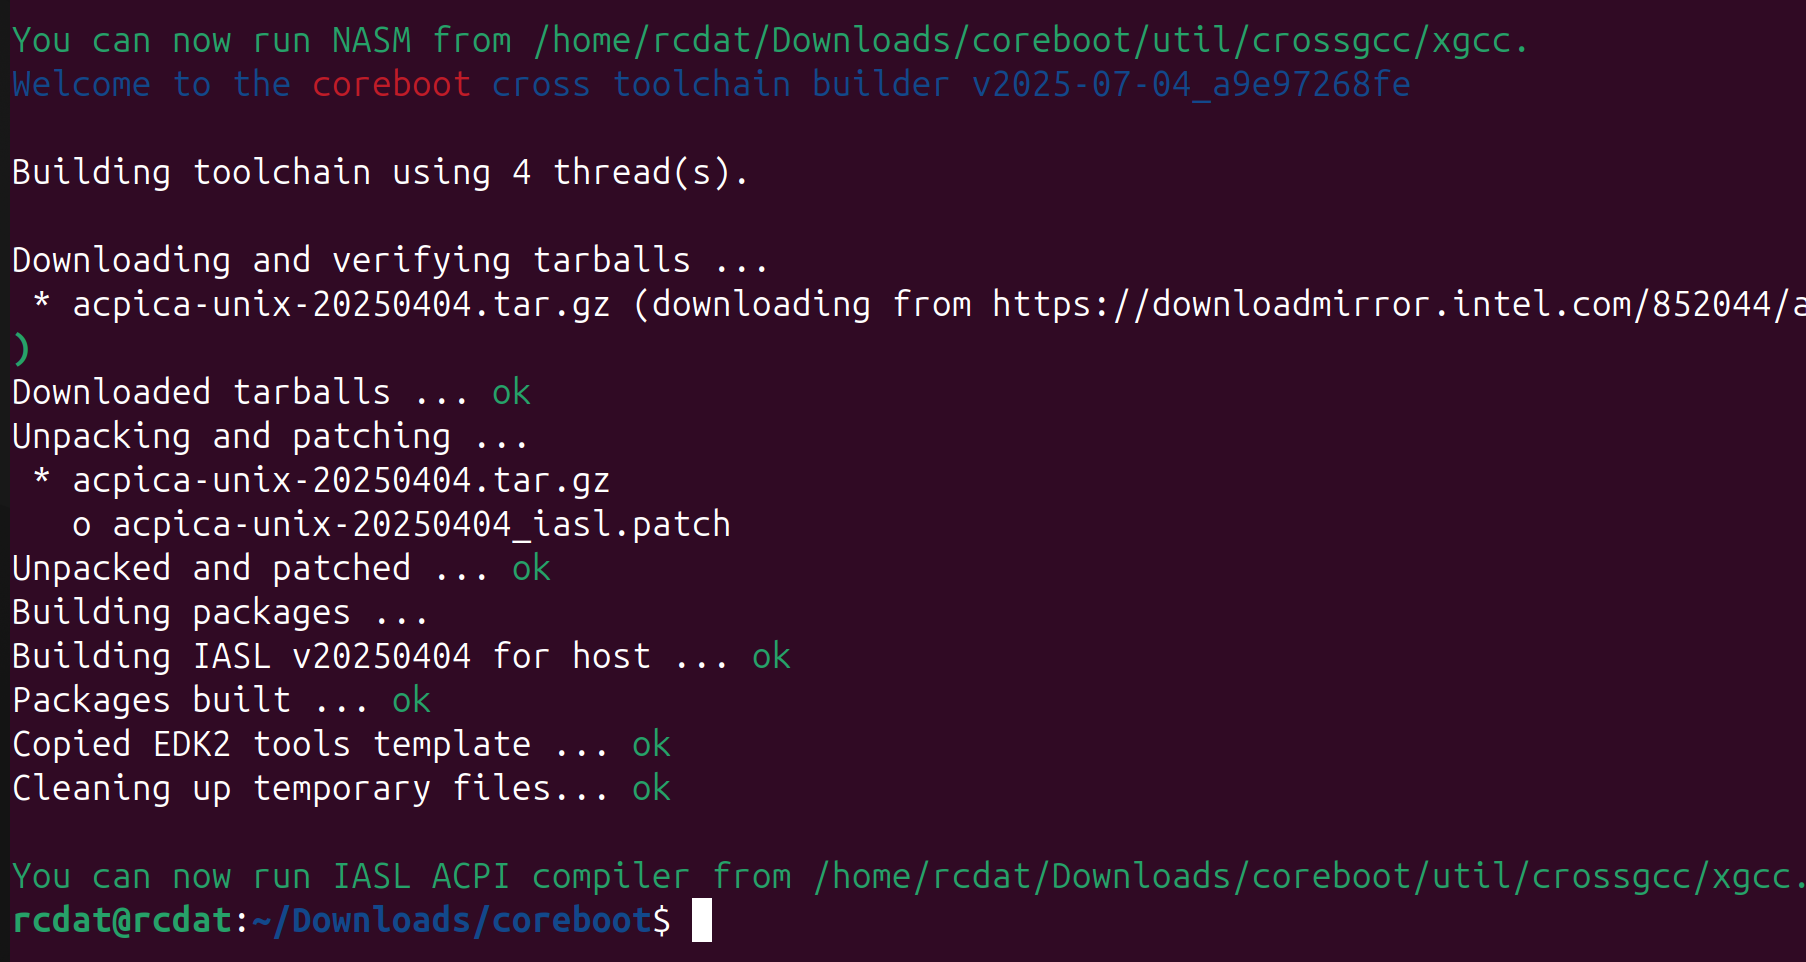
\includegraphics[width=0.8\linewidth]{images/img0}
	\end{frame}
	
	
	\begin{frame}{Installing Coreboot (Cont.)}
		\textbf{Step 6: Build the payload - coreinfo}
		
		\begin{exampleblock}{Build}
			\textcolor{blue}{\$} \texttt{sudo apt-get install -y bison} \\
				\hspace*{0em}\textcolor{blue}{\$} \texttt{make -C payloads/coreinfo} \\
		\end{exampleblock}
		
		\centering
		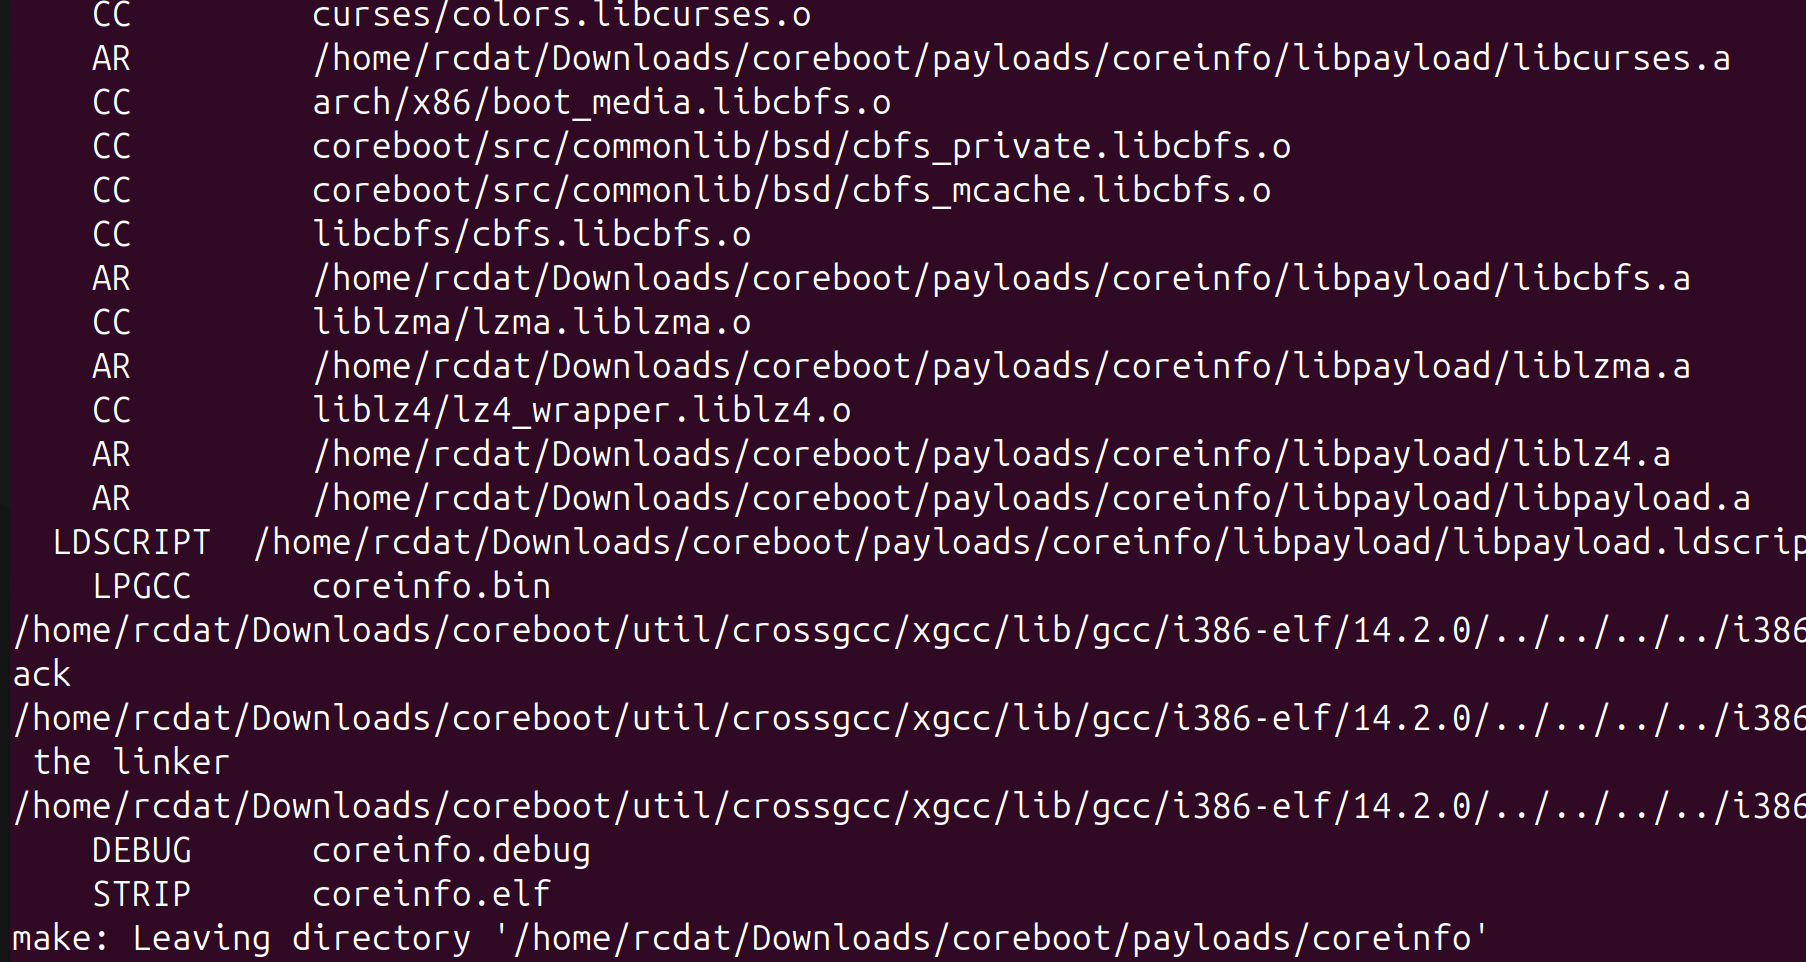
\includegraphics[width=0.8\linewidth]{images/img1}
	\end{frame}
	
	
	
	
	
	\section{Setup Complete}
	\begin{frame}{Congratulations}
		\textbf{You're Ready!}
			
		\begin{itemize}
			\item Git and Python are configured
			\item Required packages and libraries are installed
			\item Coreboot source is cloned and ready
			\item You're now ready to start building and customizing coreboot firmware!
		\end{itemize}
		
		\vspace{0.6cm}
		\centering
		\textbf{\huge \textcolor{darkgreen}{Good luck and happy hacking!}}
	\end{frame}
	
	
	
	
	
	\section{Coreboot Build Workflow}
	\begin{frame}{Coreboot Build Workflow Overview}
		\textbf{Here are the general steps to build your custom BIOS:}
		
		\begin{enumerate}
			\item Select your mainboard
			\item Choose and configure the payload (e.g., SeaBIOS, Edk2)
			\item Customize build options using \texttt{menuconfig}
			\item Build the toolchain and coreboot image
			\item Flash the image to the target board (with caution!)
			\item Verify the boot process and debug if needed
		\end{enumerate}
		
		\vspace{0.4cm}
		\centering
		\textbf{\huge \textcolor{darkgreen}{Let’s go step by step!}}
	\end{frame}
	
	
	
	
	
	
	\subsection{Board Selection}
	\begin{frame}{Select Your Mainboard}
		After downloading coreboot, the first configuration step is selecting your target mainboard.
		
		\vspace{0.3cm}
		\textbf{Step 1: Open the configuration menu}
		\begin{exampleblock}{Open coreboot menuconfig}
			\textcolor{blue}{\$} \texttt{make menuconfig}
		\end{exampleblock}
		
		\textbf{Step 2: Navigate to the mainboard selection}
		
		\begin{itemize}
			\item Choose: \texttt{Mainboard} $\rightarrow$ \texttt{Mainboard vendor}
			\item Then choose your specific board model
		\end{itemize}
		
		\vspace{0.3cm}
		\textbf{Tip:} You must know the exact vendor and model of your board before continuing.
	\end{frame}
	
	
	
	
	
	\begin{frame}{Select Your Mainboard (Cont.)}
		\centering
		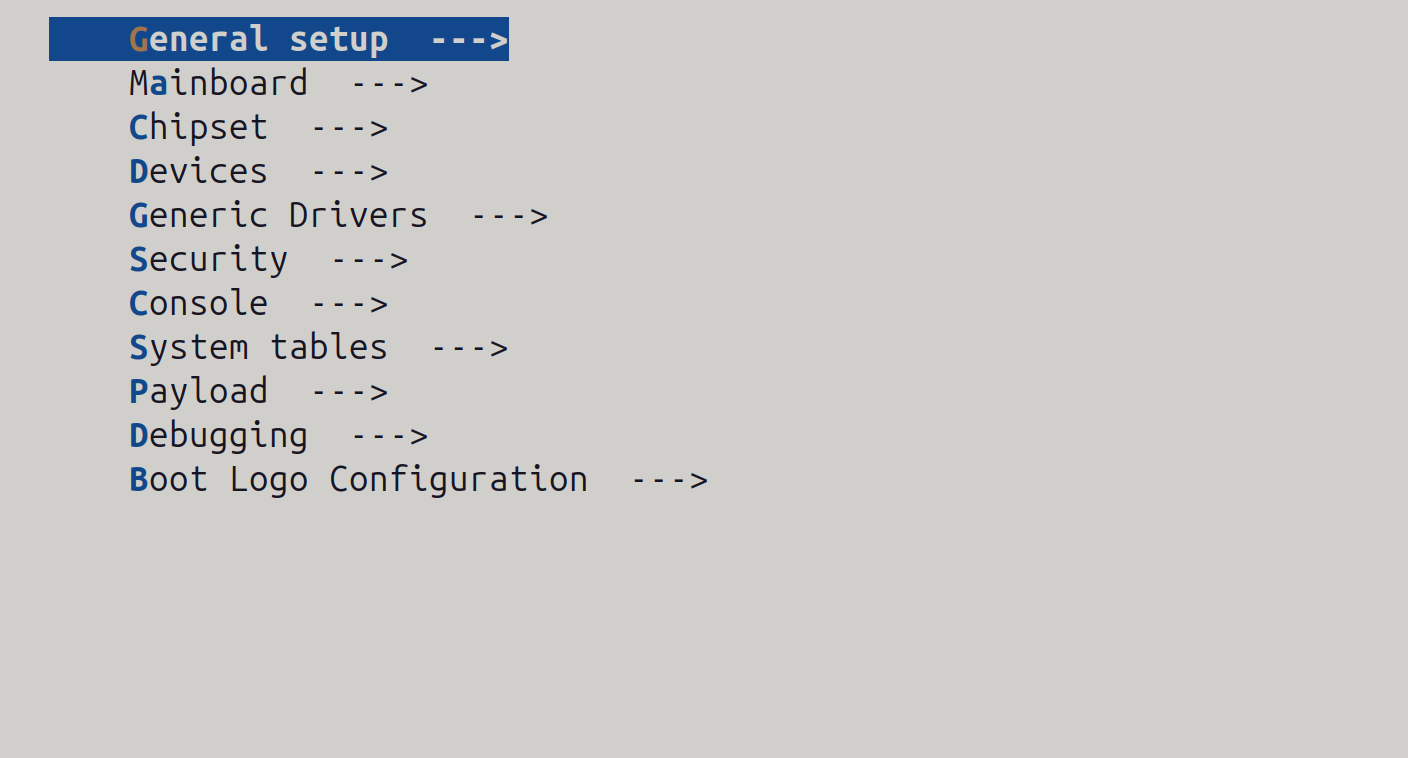
\includegraphics[width=1\linewidth]{images/img2}
	\end{frame}
	
	
	
	\begin{frame}{Select Your Mainboard (Cont.)}
		\centering
		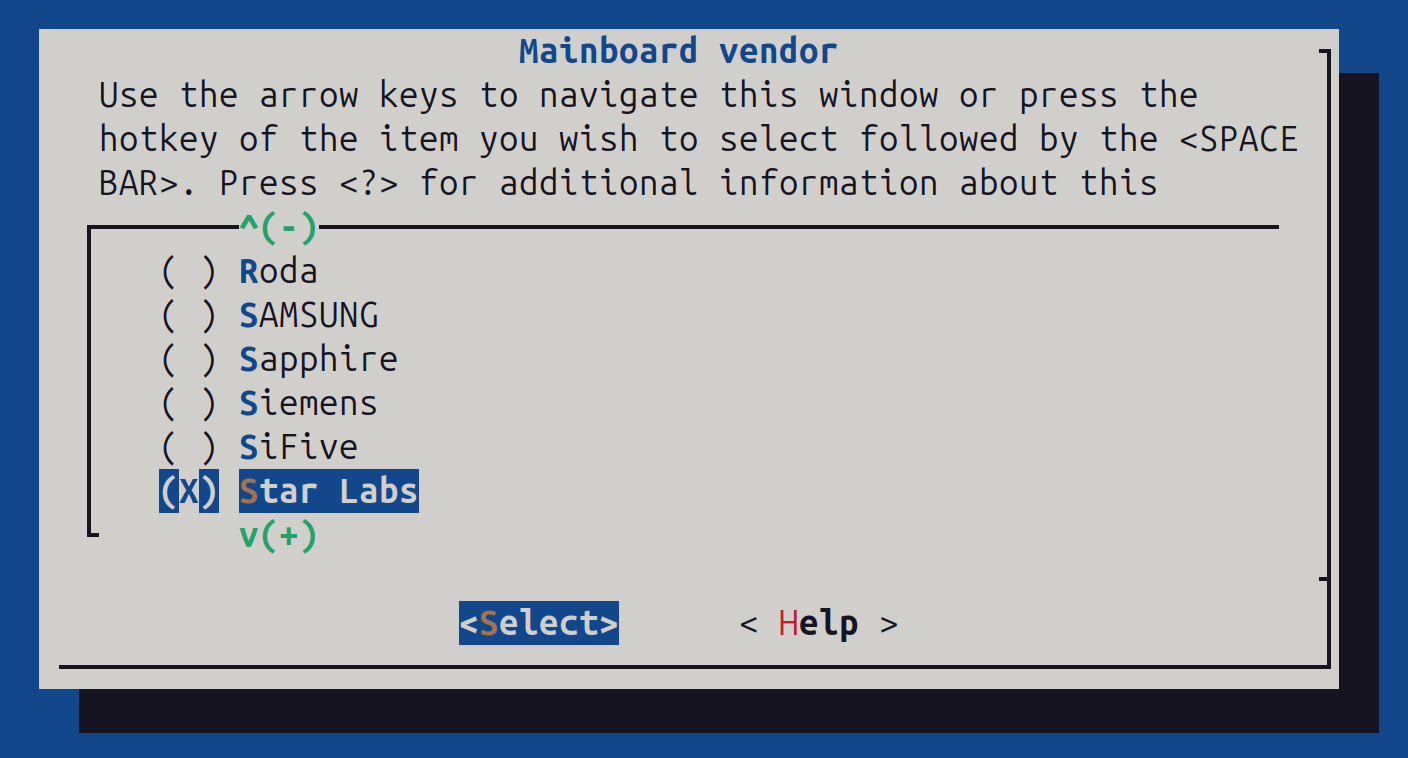
\includegraphics[width=1\linewidth]{images/img3}
	\end{frame}
	
	
	
	\begin{frame}{Select Your Mainboard (Cont.)}
		\centering
		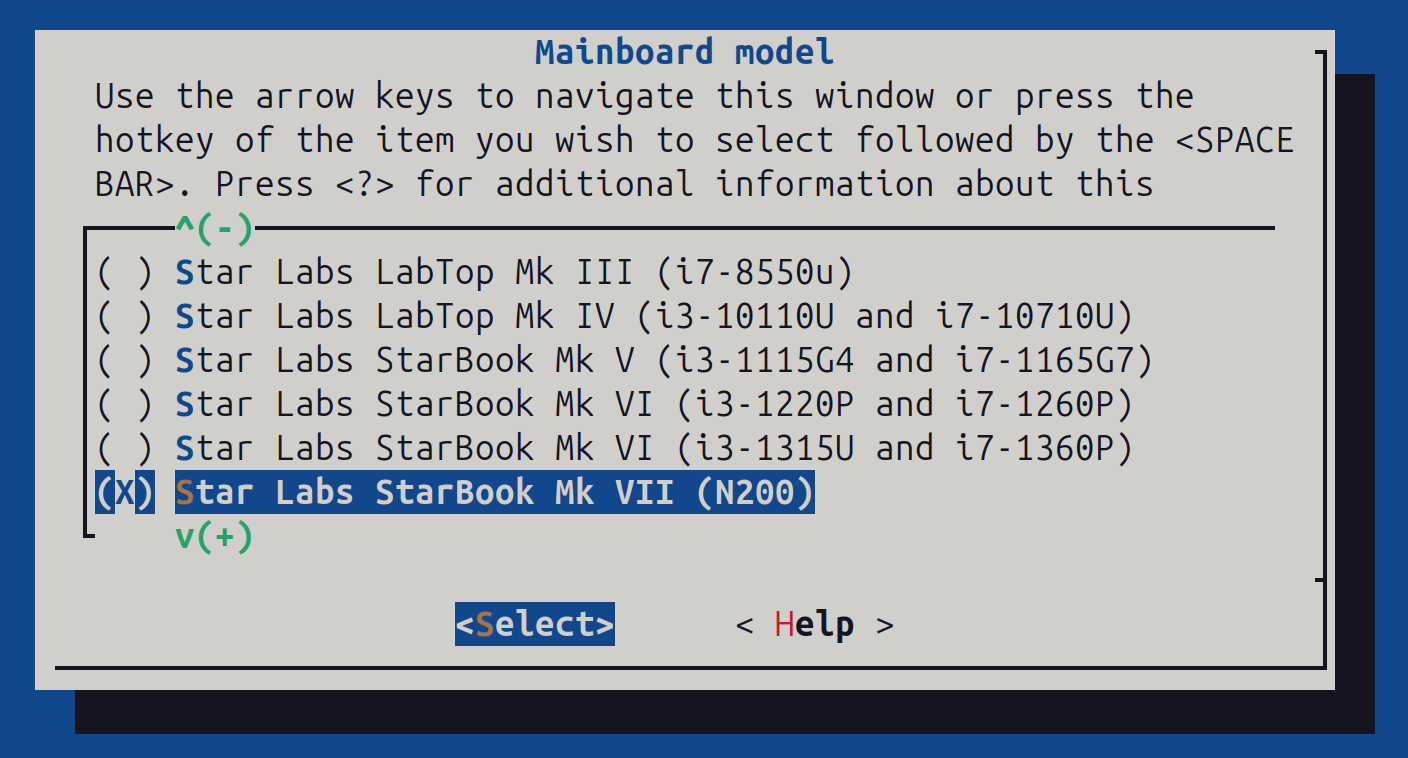
\includegraphics[width=1\linewidth]{images/img4}
	\end{frame}
	
	
	
	
	\subsection{Save Config \& Build}
	\begin{frame}{Saving Configuration and Build}
		\textbf{Step 1: Save your configuration after running \texttt{make menuconfig}}
		
		\begin{exampleblock}{Save config to default location}
			Configuration is saved to: \texttt{.config} \\ using: \texttt{make savedefconfig}
		\end{exampleblock}
		
		\textbf{Step 2: Display the saved config (optional)}
		
		\begin{exampleblock}{View config}
			\textcolor{blue}{\$} \texttt{cat defconfig} (or \texttt{cat .config})
		\end{exampleblock}
		
		\textbf{Step 3: Build coreboot}
		
		\begin{exampleblock}{Start build}
			\textcolor{blue}{\$} \texttt{make -j\$(nproc)}
		\end{exampleblock}
	\end{frame}
	
	
	
	
	
	\subsection{Fix Python Error}
	\begin{frame}{Fix Python Error}
		
		\textbf{After building, you might see below error:}
		
		\begin{exampleblock}{Error message}
			/bin/sh: 1: python: not found
		\end{exampleblock}
		
		\centering
		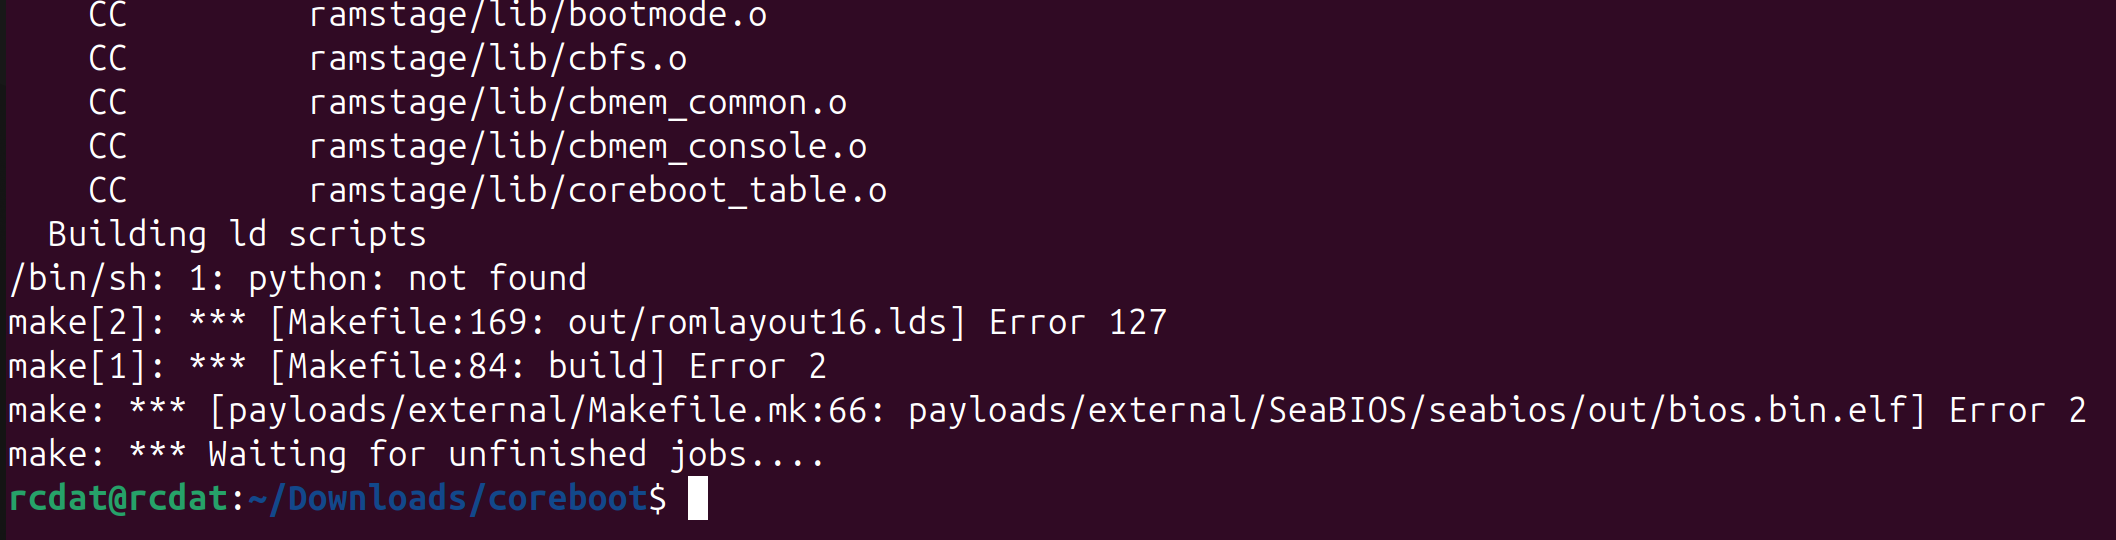
\includegraphics[width=1\linewidth]{images/img5}
	\end{frame}
	
	
	

	\begin{frame}{Fix Python Error (Cont.)}
		\textbf{Cause:}
		\begin{itemize}
			\item Some build scripts (e.g., SeaBIOS) expect the command \texttt{python} to exist.
			\item On modern Linux systems, only \texttt{python3} is installed by default.
			\item The legacy \texttt{python} command is missing, causing the build to fail.
		\end{itemize}
		
		\vspace{0.4cm}
		\textbf{Solution: Create the \texttt{python} symlink pointing to \texttt{python3}}
		
		\begin{exampleblock}{Install compatibility package}
			\textcolor{blue}{\$} \texttt{sudo apt install python-is-python3}
		\end{exampleblock}
		
		\textbf{This will make \texttt{python} point to \texttt{python3}, fixing the error.}
		
		\vspace{0.4cm}
		\textbf{Alternative (if package not available):}
		\begin{exampleblock}{Manual symlink (advanced)}
			\textcolor{blue}{\$} \texttt{sudo ln -s /usr/bin/python3 /usr/bin/python}
		\end{exampleblock}
	\end{frame}
	
	
	
	
	
	
	
	\subsection{Fix EDK2 Build Error}
	\begin{frame}{Fixing EDK2 Payload Build Error}
		\textbf{Problem: Missing tools required by EDK2 (TianoCore UEFI payload)}
		
		\textbf{Common Errors:}
		\begin{exampleblock}{NASM not found}
			EDK2: Checking nasm:        Not found! \\
			ERROR: Please install nasm.
		\end{exampleblock}
		
		\begin{exampleblock}{Missing NSS (optional)}
			Missing NSS. PKCS11 signing not supported. Install libnss3 to enable this feature.
		\end{exampleblock}
	\end{frame}
	
	
	
	
	\begin{frame}{Fixing EDK2 Payload Build Error (Cont.)}
		\centering
		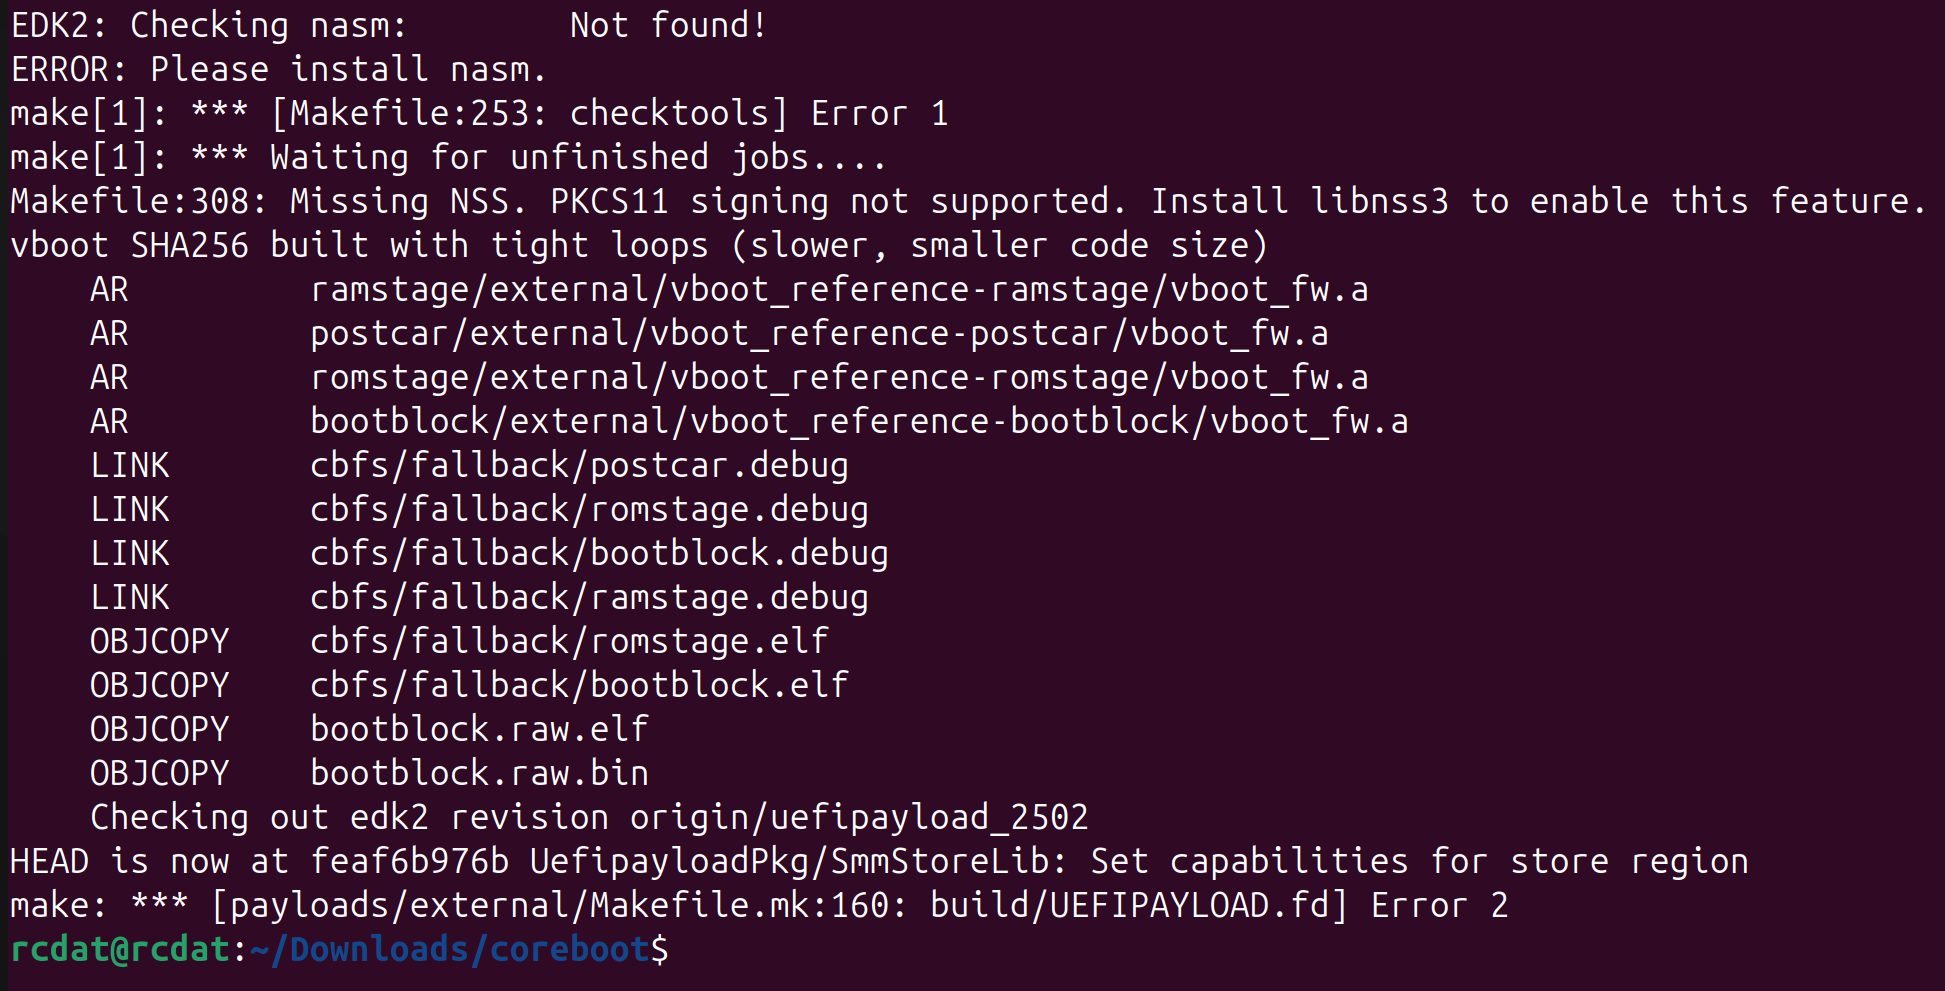
\includegraphics[width=1\linewidth]{images/img6}
	\end{frame}
	
	
	
	\begin{frame}{Fixing EDK2 Payload Build Error (Cont.)}
		\vspace{0.3cm}
		\textbf{Solution: Install required packages}
		
		\begin{exampleblock}{Fix command (Ubuntu/Debian)}
			\textcolor{blue}{\$} \texttt{sudo apt install nasm uuid-dev iasl build-essential libnss3}
		\end{exampleblock}
		
		\textbf{Then rebuild again:}
		
		\begin{exampleblock}{Retry the build}
			\textcolor{blue}{\$} \texttt{make -j\$(nproc)}
		\end{exampleblock}
	\end{frame}
	
	
	
	
	
	\subsection{Build Complete}
	\begin{frame}{Build Successful}
		\begin{block}{Congratulations!}
			Coreboot has been successfully built with your selected configuration and payload.
		\end{block}
		
		\centering
		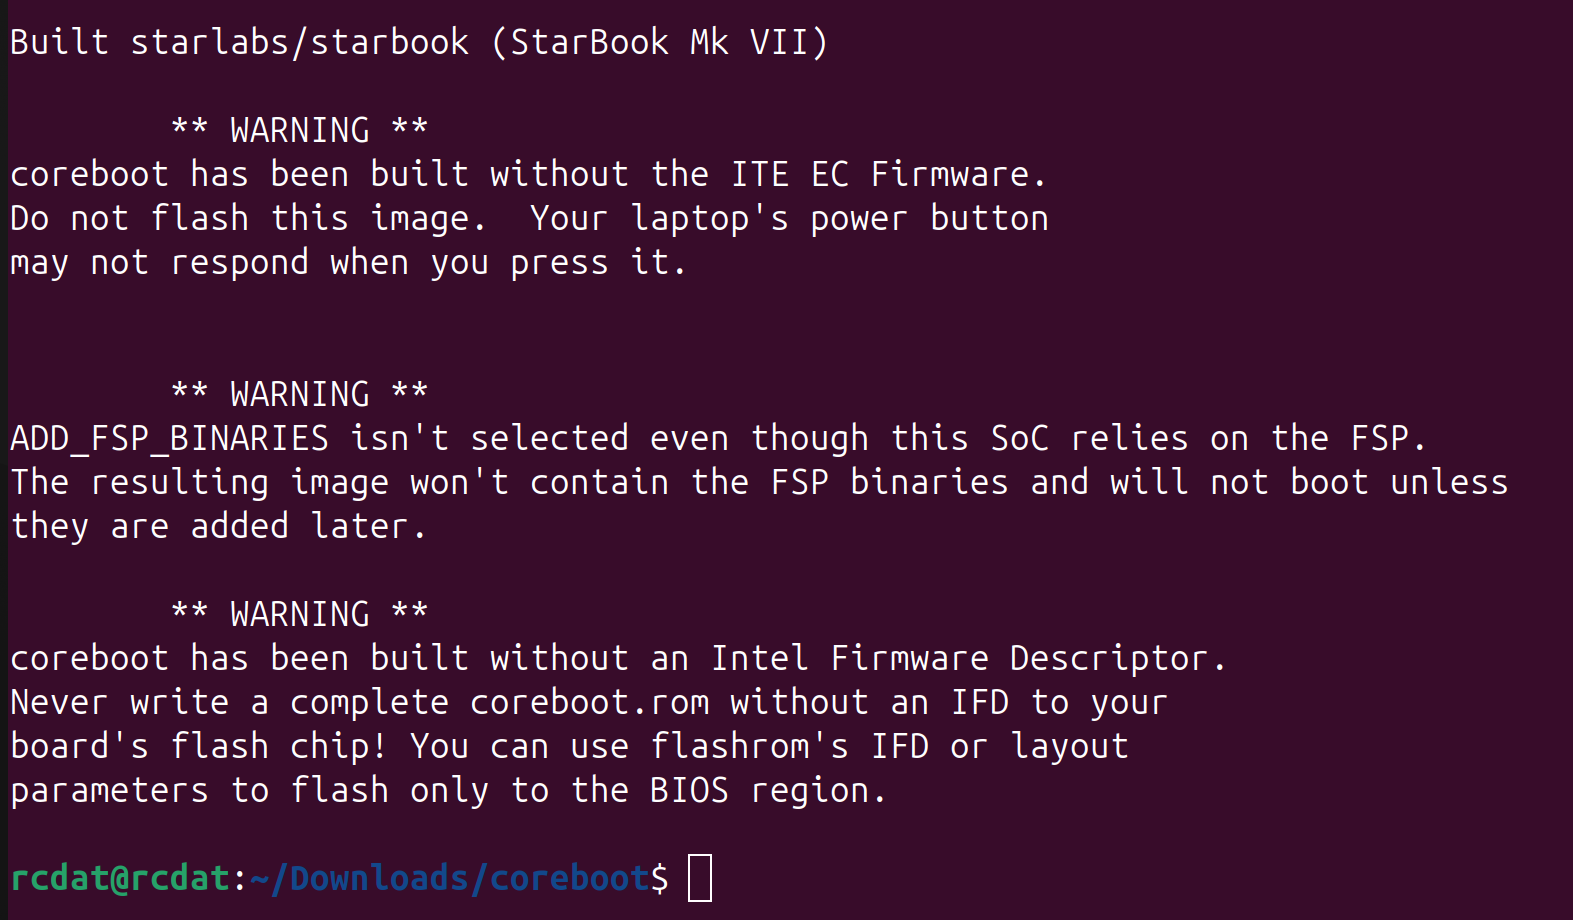
\includegraphics[width=0.8\linewidth]{images/img7.png} 
		
		\begin{exampleblock}{Output ROM Image}
			\texttt{build/coreboot.rom}
		\end{exampleblock}
	\end{frame}
	
	
	
	
	
	
	\begin{frame}{Post-Build Warnings (Read Carefully)}
		\begin{itemize}
			\item \textbf{Missing ITE EC Firmware:} Power button may stop working. Do not flash this image as-is.
			\item \textbf{FSP Binaries Not Included:} SoC requires FSP. Image will not boot without it.
			\item \textbf{No Intel Firmware Descriptor (IFD):} Never flash full ROM without IFD! Use \texttt{flashrom} with layout or region flags.
		\end{itemize}
		
		\vspace{0.4cm}
		\textbf{\textcolor{red}{Fix these issues before flashing the image.}}
	\end{frame}
	
	
	
	
	
	\begin{frame}{Adding FSP and IFD to Your Coreboot Image}
		\textbf{To ensure your image boots safely:}
		
		\begin{itemize}
			\item \textbf{FSP (Firmware Support Package):}
			\begin{itemize}
				\item Download FSP binary from Intel or vendor.
				\item Enable \texttt{ADD\_FSP\_BINARIES} in \texttt{make menuconfig}.
				\item Place FSP file in \texttt{3rdparty/blobs/...} as instructed.
			\end{itemize}
			
			\item \textbf{IFD (Intel Firmware Descriptor):}
			\begin{itemize}
				\item Extract it from your original ROM using:
				\begin{exampleblock}{Extract IFD from dump}
					\textcolor{blue}{\$} \texttt{ifdtool -x original.rom}
				\end{exampleblock}
				\item Merge it into your Coreboot build using:
				\begin{exampleblock}{Insert IFD}
					\textcolor{blue}{\$} \texttt{ifdtool -i fd:flashregion\_0\_descriptor.bin coreboot.rom}
				\end{exampleblock}
			\end{itemize}
		\end{itemize}
		
		\textbf{Only flash after confirming both FSP and IFD are present.}
	\end{frame}
	
	
	
	
	\section{Flashing Coreboot Image}
	\begin{frame}{Flashing Coreboot Image Safely}
		\textbf{Never overwrite the entire flash chip if IFD is missing!}
		
		\textbf{Step 1: Dump and inspect your original ROM}
		\begin{exampleblock}{Backup current firmware}
			\textcolor{blue}{\$} \texttt{flashrom -p <programmer> -r [YOUR/PATH/]/original.rom}
		\end{exampleblock}
		\vspace*{2.8em}
		\textbf{Step 2: Extract and reuse layout}
		\begin{exampleblock}{Extract layout (optional)}
			\textcolor{blue}{\$} \texttt{ifdtool -x original.rom}
		\end{exampleblock}
	\end{frame}
	
	
	
	\begin{frame}{Flashing Coreboot Image Safely (Cont.)}
		\textbf{Step 3: Flash only the BIOS region}
		\begin{exampleblock}{Flash BIOS region safely}
			\textcolor{blue}{\$} \texttt{flashrom -p <programmer> -w coreboot.rom \\
				\hspace*{2.8em}--ifd -i bios}
		\end{exampleblock}
		
		\vspace{1cm}
		\textbf{Use external flasher (e.g. CH341A) if unsure or testing first time.}
		
	\end{frame}
	
	
	
	
	
	\section{First Boot: Verifying Coreboot Works}
	\begin{frame}{First Boot: Verifying Coreboot Works}
		\textbf{After flashing, verify that Coreboot boots successfully.}
		
		\textbf{Signs of success:}
		\begin{itemize}
			\item System powers on and screen initializes
			\item Payload (e.g., SeaBIOS, Tianocore) shows a boot screen
			\item You can boot into OS or see a boot device menu
		\end{itemize}
		
		\textbf{For deeper verification:}
		\begin{itemize}
			\item Use UART/serial output for debug logs
			\item Check if EC (Embedded Controller) responds to power/reset
			\item Confirm BIOS region was correctly flashed with \texttt{flashrom -v}
		\end{itemize}
	\end{frame}
	
	
	
	\begin{frame}{First Boot: Verifying Coreboot Works (Cont.)}
		\textbf{If system does not boot:}
		\begin{itemize}
			\item Reflash original firmware backup (Externally)
			\item Recheck EC firmware, FSP, and IFD
			\item Review serial logs if available
		\end{itemize}
	\end{frame}
	
	
	
	
	
	
	\begin{frame}{Questions?}
		\centering
		\Huge \textbf{Any Questions?} \\[0.8cm]
		
		\Large Thank you for your attention! \\[0.6cm]
		
		\normalsize
		\textbf{Slides available at:} \\
		\texttt{\href{https://github.com/rezaAdinepour/ISC-Workshop.git}{\textcolor{blue}{https://github.com/rezaAdinepour/ISC-Workshop.git}}}
	\end{frame}
	
	
	
	
\end{document}
